
We implemented kcores method
and tested other algorithms that are already implemented in the system with unit tests and other datasets from SNAP.

Figures below give the degree distribution and pagerank result of two dataset from SNAP. We can find that the degree distribution and pagerank results are consistent with the power law as nodes or pages with higher degree or rank have a small number while nodes or pages with lower degree or rank have a large number.
You can also find the detailed results in the output folder, which contains csv files for the results of belief propagation, connected components, node degrees, degree distribution, eigen values, k-core connected components, pagerank results, radius, etc. 


\begin{figure}[H]
\begin{center}
\begin{tabular}{cc}
     % uncomment the next lines, and give the right ps files
     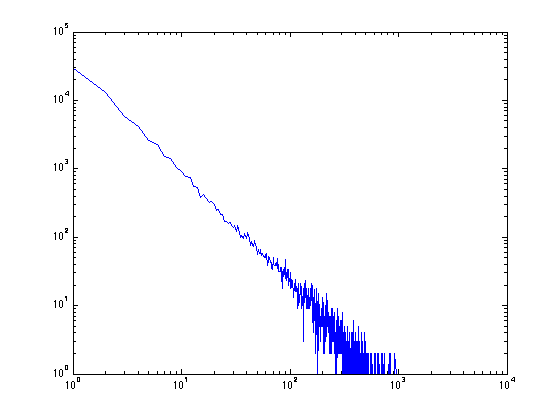
\includegraphics[width=0.3\textwidth]{FIG/soc-degreedist.png} &
     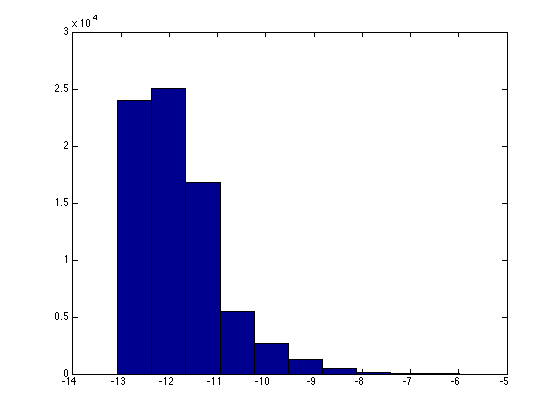
\includegraphics[width=0.3\textwidth]{FIG/soc-pagerank.png} \\
\end{tabular}
\caption{Degree Distribution(a) and PageRank(b) for Dataset SOC-Epinions1}

\begin{tabular}{cc}
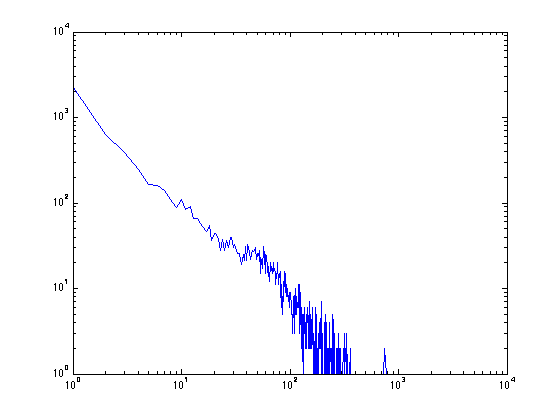
\includegraphics[width=0.3\textwidth]{FIG/wiki-degreedist.png} &
     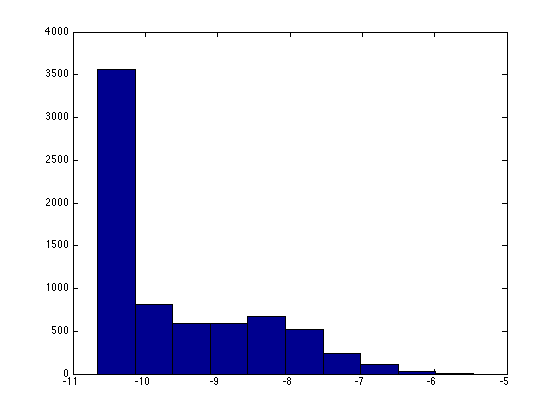
\includegraphics[width=0.3\textwidth]{FIG/wiki-pagerank.png} \\

     %\psfig{figure=FIG/plot.ps,width=2in} \\
     % \psfig{figure=FIG/data.ps,width=2in} &
     % \psfig{figure=FIG/plot.ps,width=2in} \\
    (a) & (b)
\end{tabular}
\caption{Degree Distribution(a) and PageRank(b) for Dataset wiki-Vote}

\end{center}
\end{figure}

The figures below also include the degree distribution, connected components, k=5 cores algorithm results on the 5 unit tests.
As the unit tests are small, there is no nodes in the tests that satisfy k=5 cores, so the output result for these 5 
unit tests are empty. 
However, you can find the node id, component id pairs in the stdout output from console or in the kcorecomponent.csv file, which shows that the k-core
algorithm works as it claims to find correct coreness subgraphs.

\begin{figure}[H]
\begin{center}
\begin{tabular}{cc}
     % uncomment the next lines, and give the right ps files
     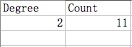
\includegraphics[width=0.3\textwidth]{FIG/1dd.jpg} &
     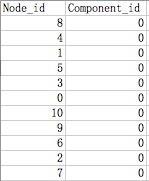
\includegraphics[width=0.3\textwidth]{FIG/1cc.jpg} \\
\end{tabular}
\caption{Degree Distribution(a), connected components(b) for Dataset1}
\end{center}
\end{figure}

\begin{figure}[H]
\begin{center}
\begin{tabular}{cc}
     % uncomment the next lines, and give the right ps files
     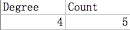
\includegraphics[width=0.3\textwidth]{FIG/2dd.jpg} &
     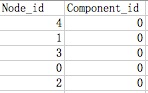
\includegraphics[width=0.3\textwidth]{FIG/2cc.jpg} \\
\end{tabular}
\caption{Degree Distribution(a), connected components(b) for Dataset2}
\end{center}
\end{figure}

\begin{figure}[H]
\begin{center}
\begin{tabular}{cc}
     % uncomment the next lines, and give the right ps files
     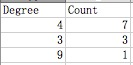
\includegraphics[width=0.3\textwidth]{FIG/3dd.jpg} &
     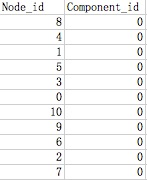
\includegraphics[width=0.3\textwidth]{FIG/3cc.jpg} \\
\end{tabular}
\caption{Degree Distribution(a), connected components(b) for Dataset3}
\end{center}
\end{figure}

\begin{figure}[H]
\begin{center}
\begin{tabular}{cc}
     % uncomment the next lines, and give the right ps files
     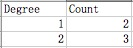
\includegraphics[width=0.3\textwidth]{FIG/4dd.jpg} &
     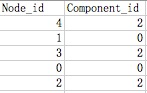
\includegraphics[width=0.3\textwidth]{FIG/4cc.jpg} \\
\end{tabular}
\caption{Degree Distribution(a), connected components(b) for Dataset4}
\end{center}
\end{figure}

\begin{figure}[H]
\begin{center}
\begin{tabular}{cc}
     % uncomment the next lines, and give the right ps files
     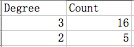
\includegraphics[width=0.3\textwidth]{FIG/5dd.jpg} &
     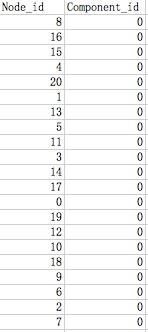
\includegraphics[width=0.3\textwidth]{FIG/5cc.jpg} \\
\end{tabular}
\caption{Degree Distribution(a) connected components(b) for Dataset5}
\end{center}
\end{figure}


We build index for algorithms Degree Distribution, K-core, Pagerank, Connected Components, All Radius, Eigen Value Computation on ten datasets:as-skitter.ungraph-75000, ca-AstroPh, cit-HepPh, cit-HepTh, com-amazon.ungraph-75000, com-dblp.ungraph-75000, email-Enron.ungraph, email-EuAll,p2p-Gnutella31, soc-Slashdot0811-75000.

We first conducted some simple tests to make sure that creating index can lead to performance improvement.
For example, 
Degree Distribution:(no index on node degree), run time is 147.476911545
Degree Distribution:(index on node degree (in degree, out degree)), run time is 346.571922302
From the experiment, create index does consume system resources and it will make performance worse in general if we
created index and used it only once.
However, 
Degree Distribution:(no index on node degree)(run 10 times), run time is 2091.14193916,
Degree Distribution:(index on node degree (in degree, out degree))(run 10 times, 1 time create index), run time is 1351.35889053.
From the experiment, create index will improve performance in general if we created index and used it later a lot.
Also, for a certain algorithm, create index for some tables like GMNODES are expensive, but if re run all the algorithms,or use the algorithm multiple times, then the cost of creating index on tables like GMNODES will be worth the effort.

This is the general intuitive for us to choose on which table and which column to create index and avoid some unnecessay tests.

We compared building index for different tables on different columns for each algorithm and get the following figures below. 

\begin{figure}[H]
\begin{center}
\begin{tabular}{cc}
     % uncomment the next lines, and give the right ps files
     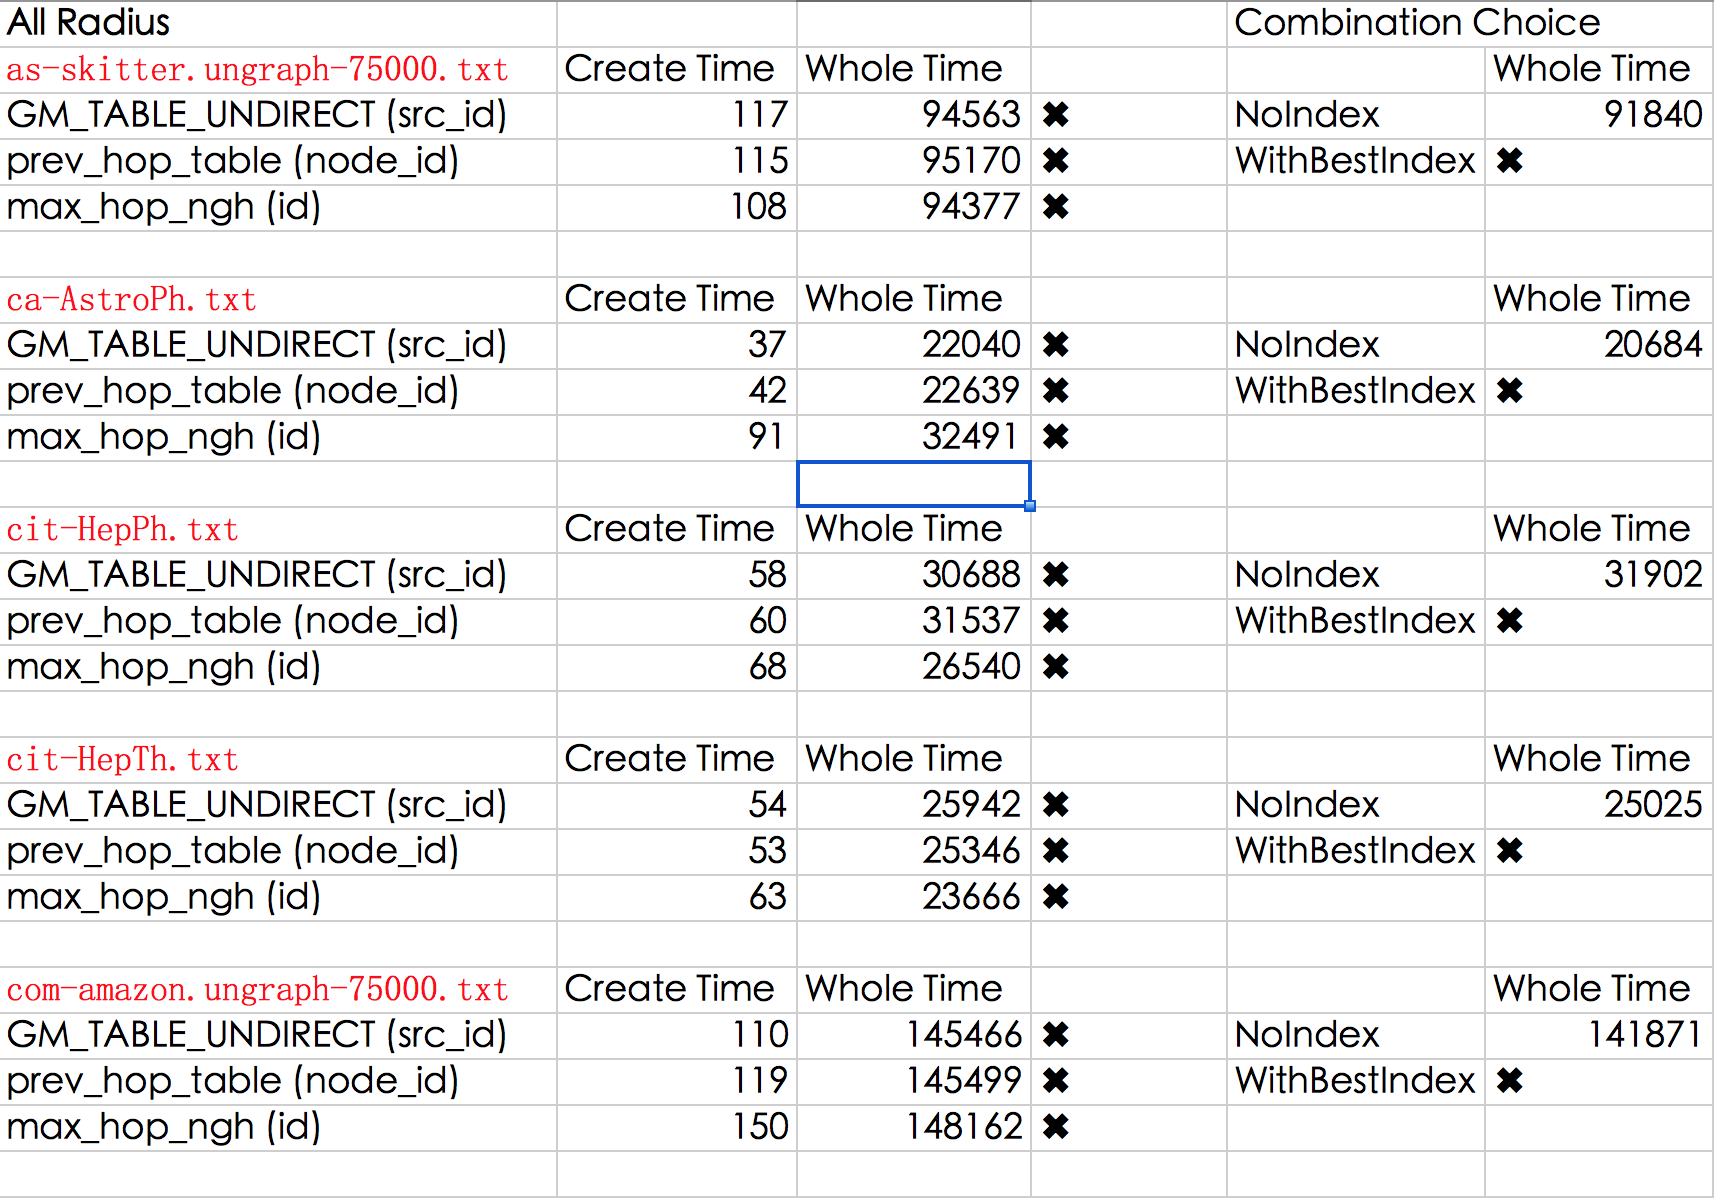
\includegraphics[width=1.0\textwidth]{FIG/AllRadius1.png} \\
     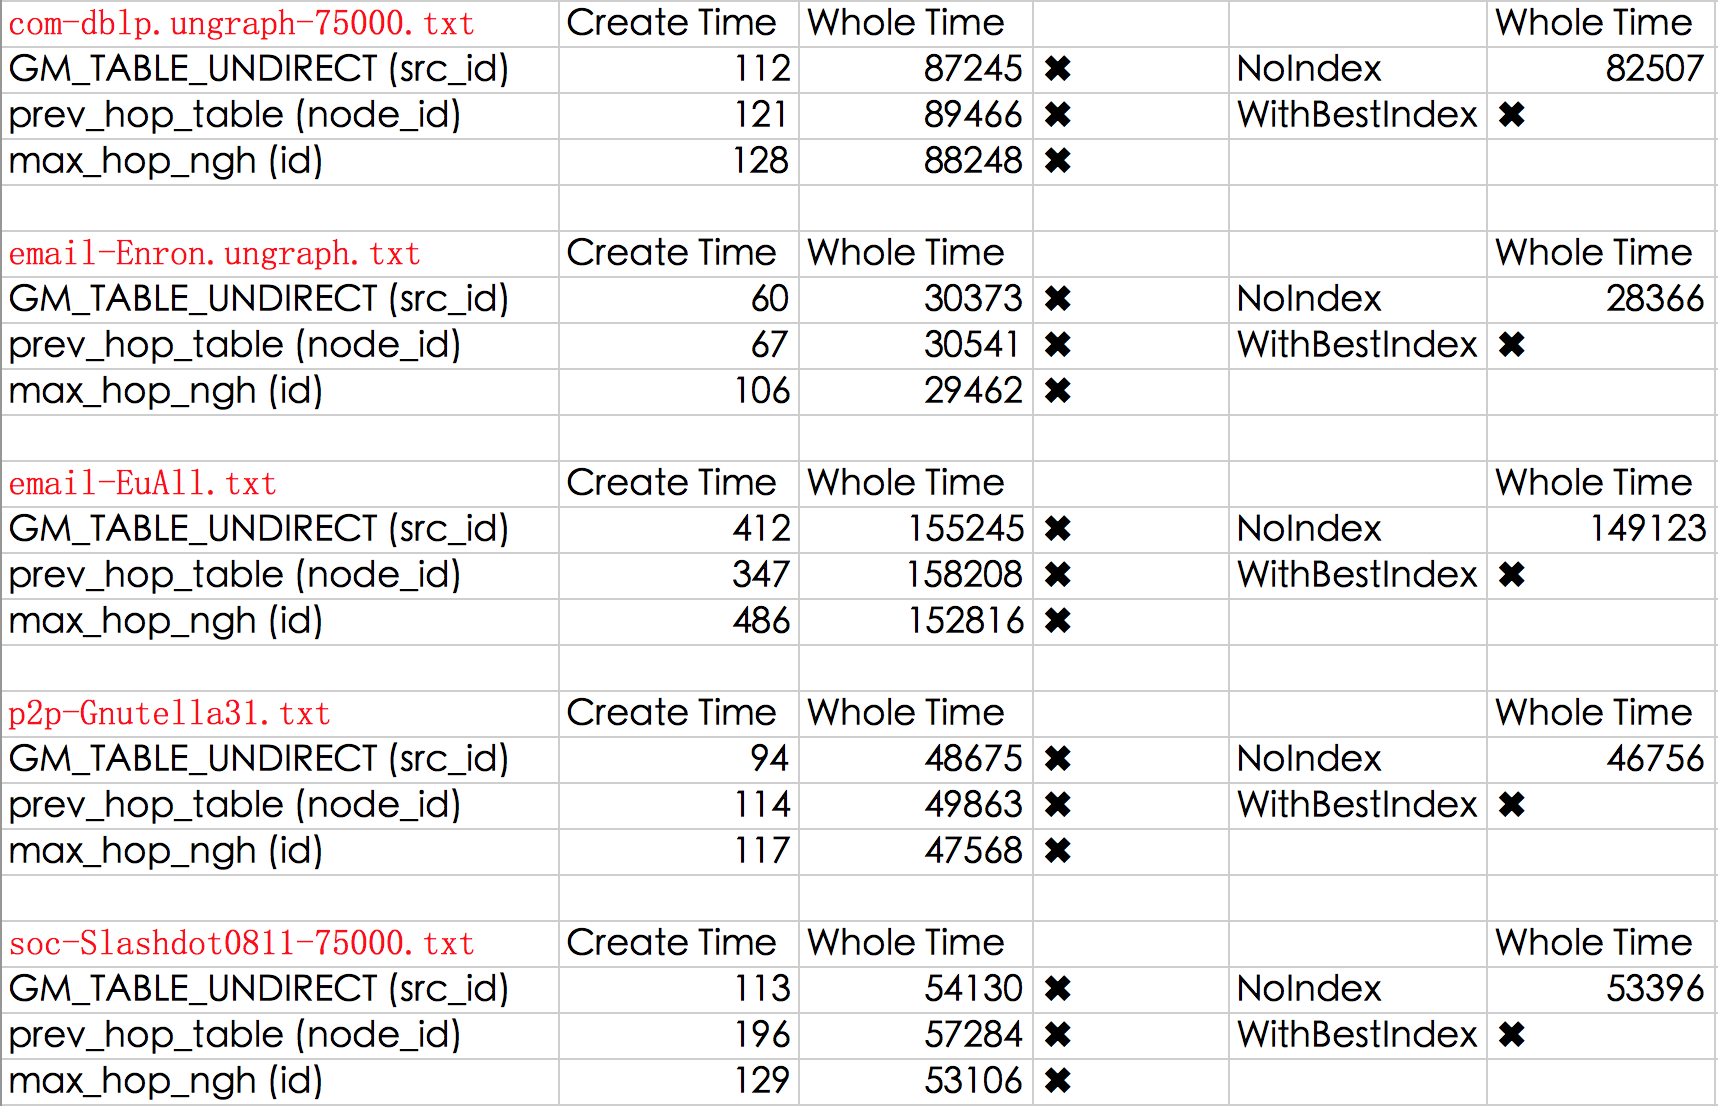
\includegraphics[width=1.0\textwidth]{FIG/AllRadius2.png} \\
\end{tabular}
\caption{Creating Index Experiments on All Radius Algorithm}
\end{center}
\end{figure}

\begin{figure}[H]
\begin{center}
\begin{tabular}{cc}
     % uncomment the next lines, and give the right ps files
     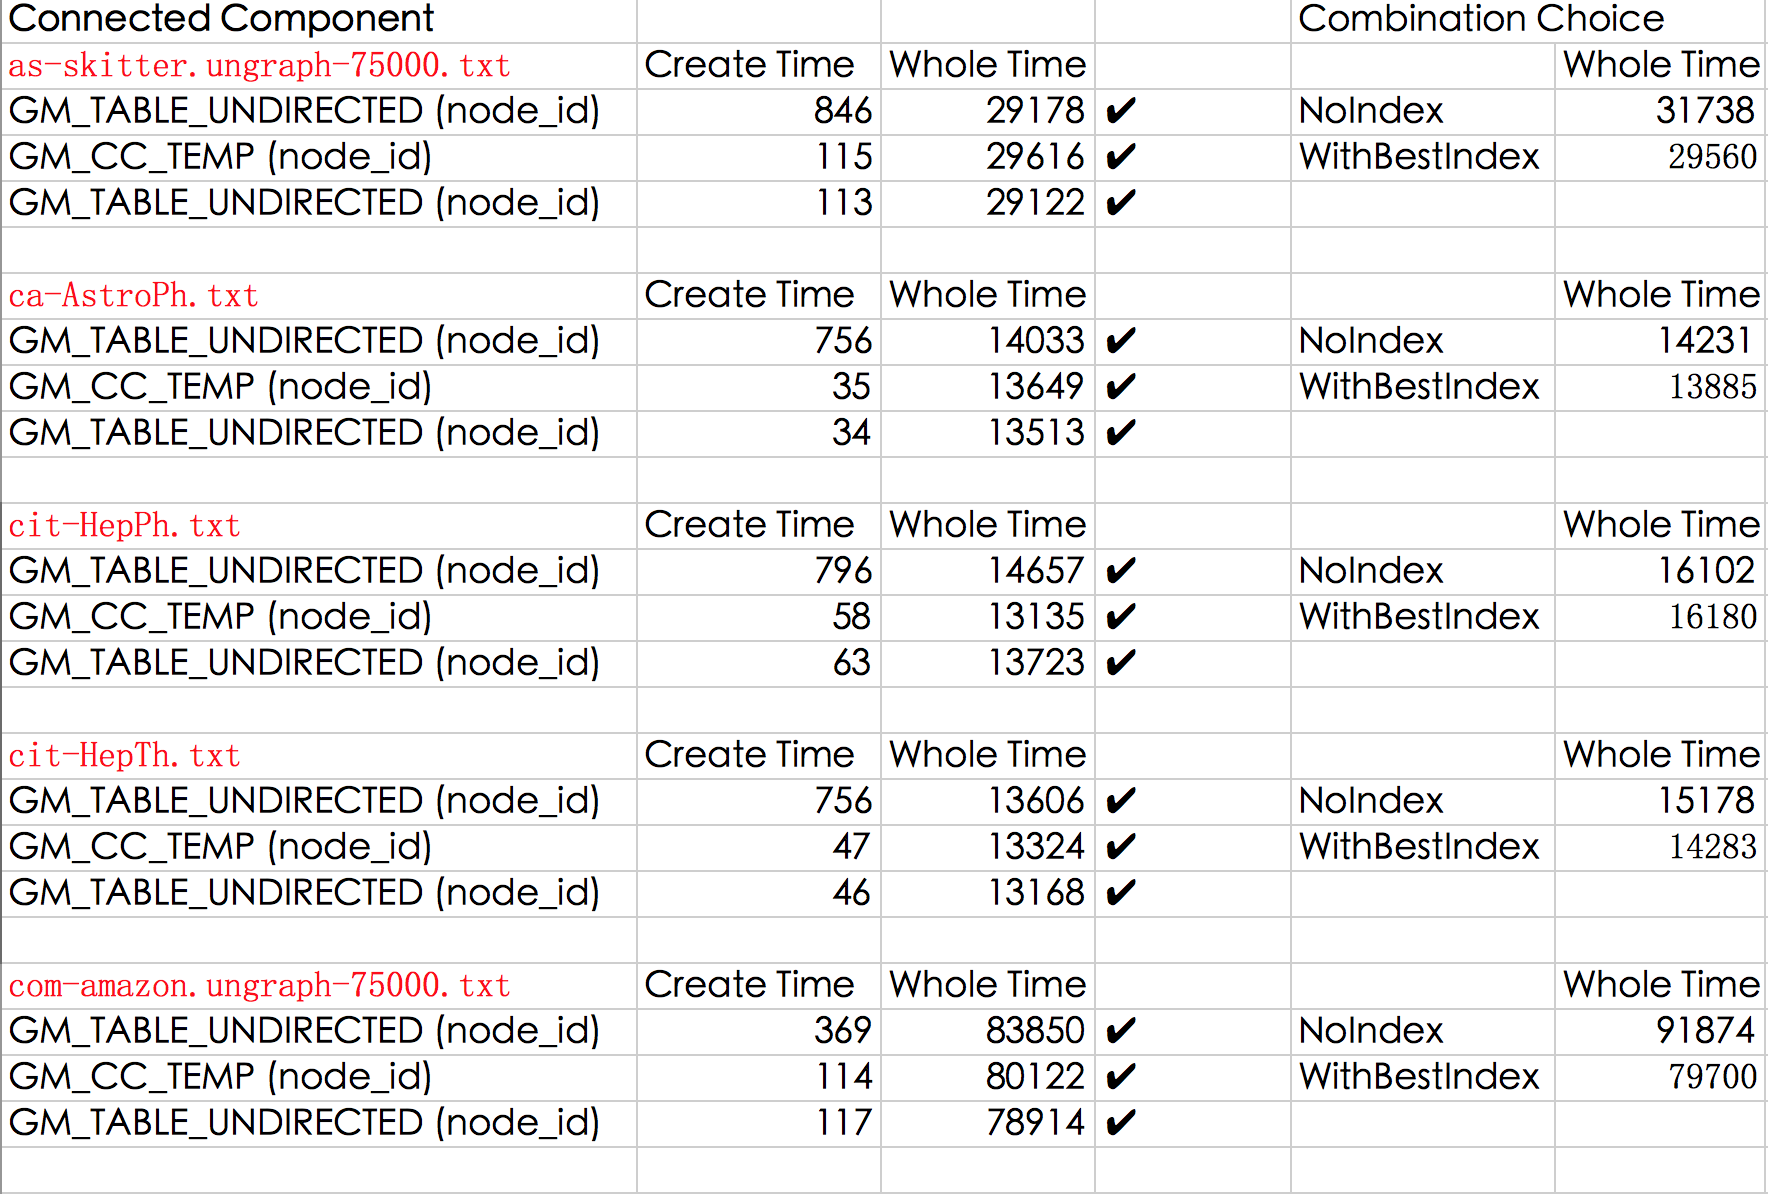
\includegraphics[width=1.0\textwidth]{FIG/CC1.png} \\
     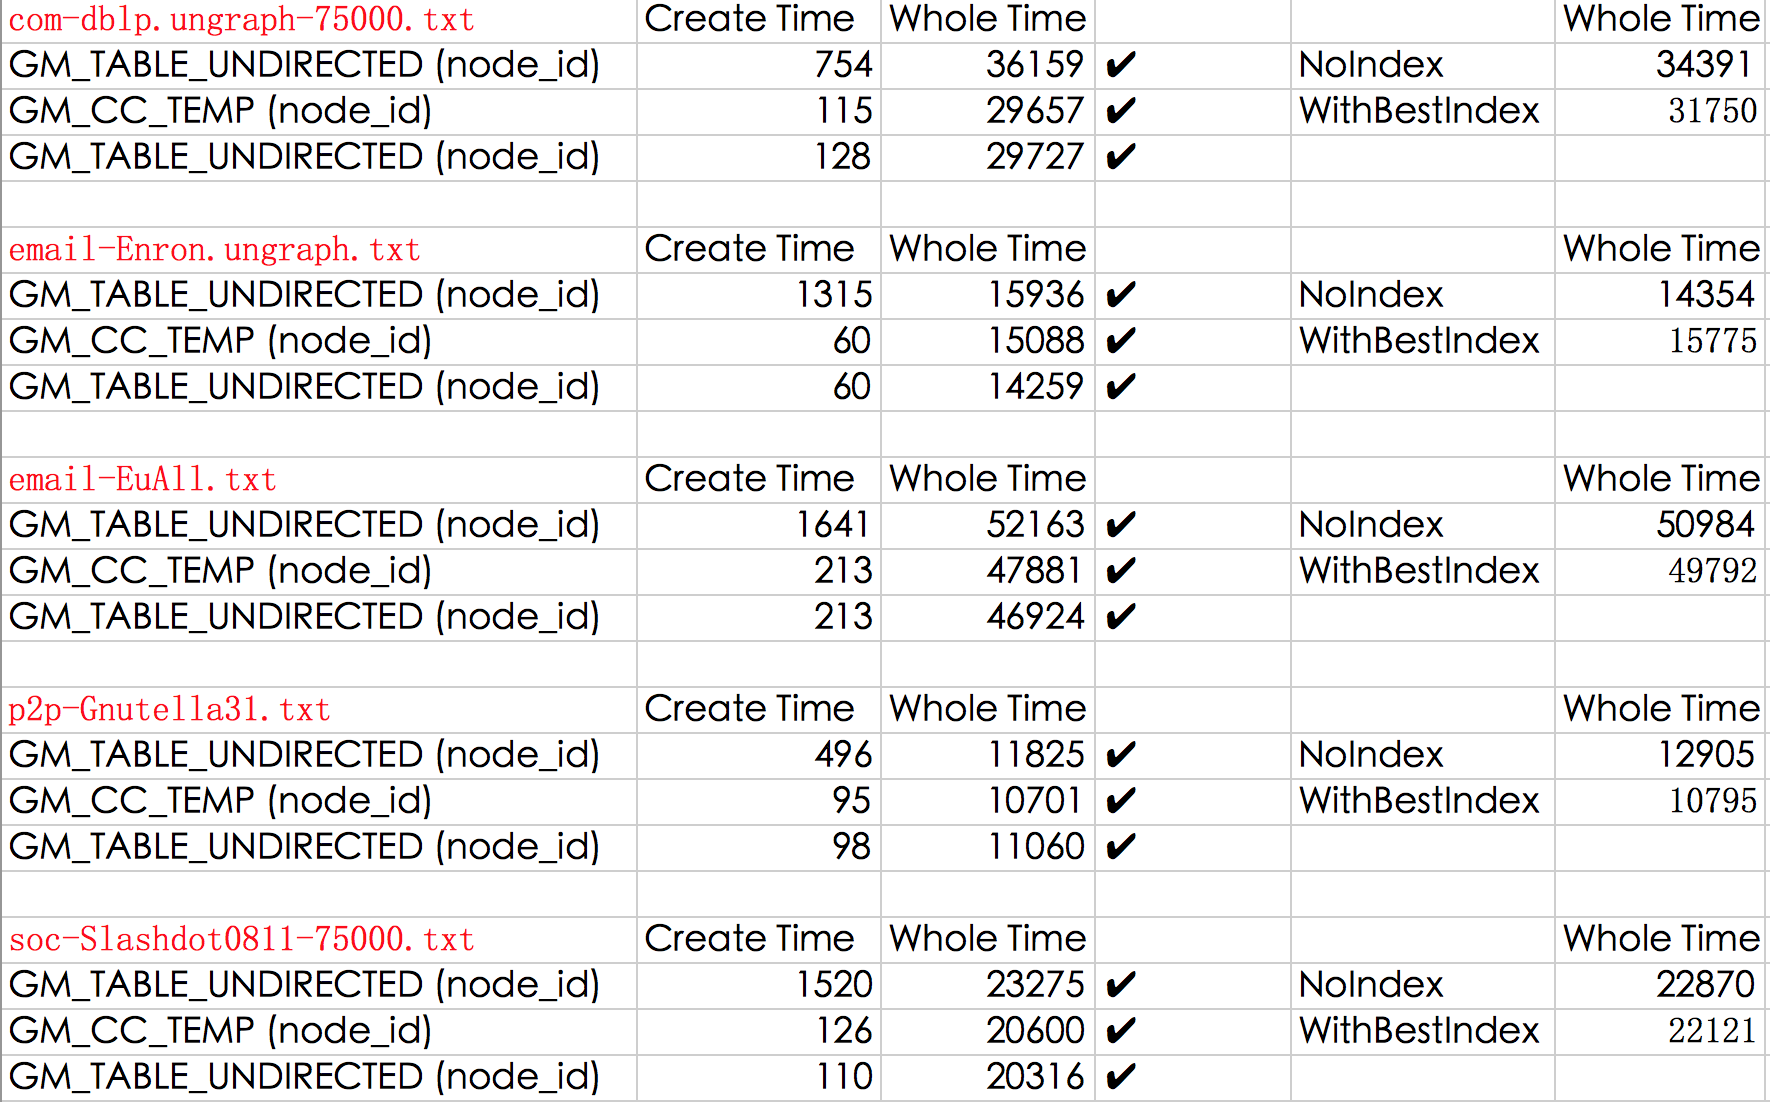
\includegraphics[width=1.0\textwidth]{FIG/CC2.png} \\
\end{tabular}
\caption{Creating Index Experiments on Connected Components Algorithm}
\end{center}
\end{figure}

\begin{figure}[H]
\begin{center}
\begin{tabular}{cc}
     % uncomment the next lines, and give the right ps files
     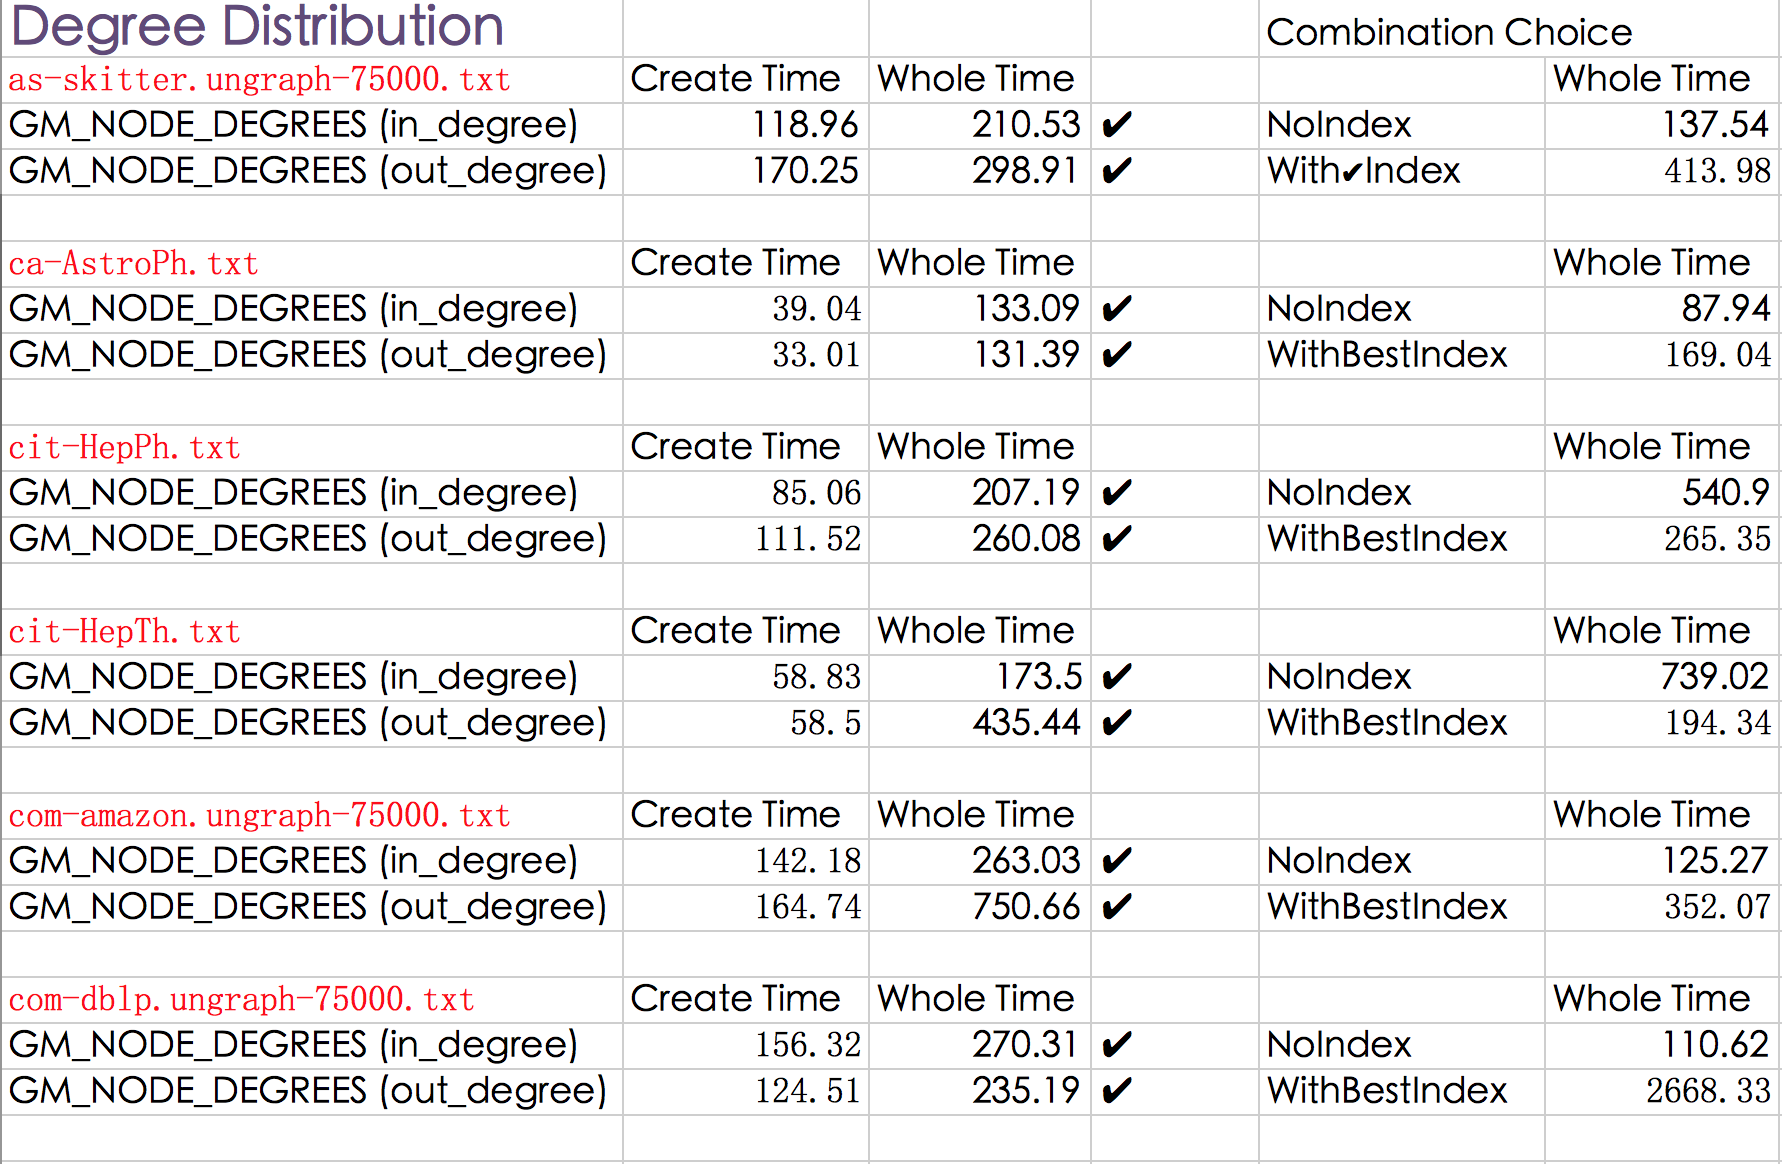
\includegraphics[width=1.0\textwidth]{FIG/DD1.png} \\
     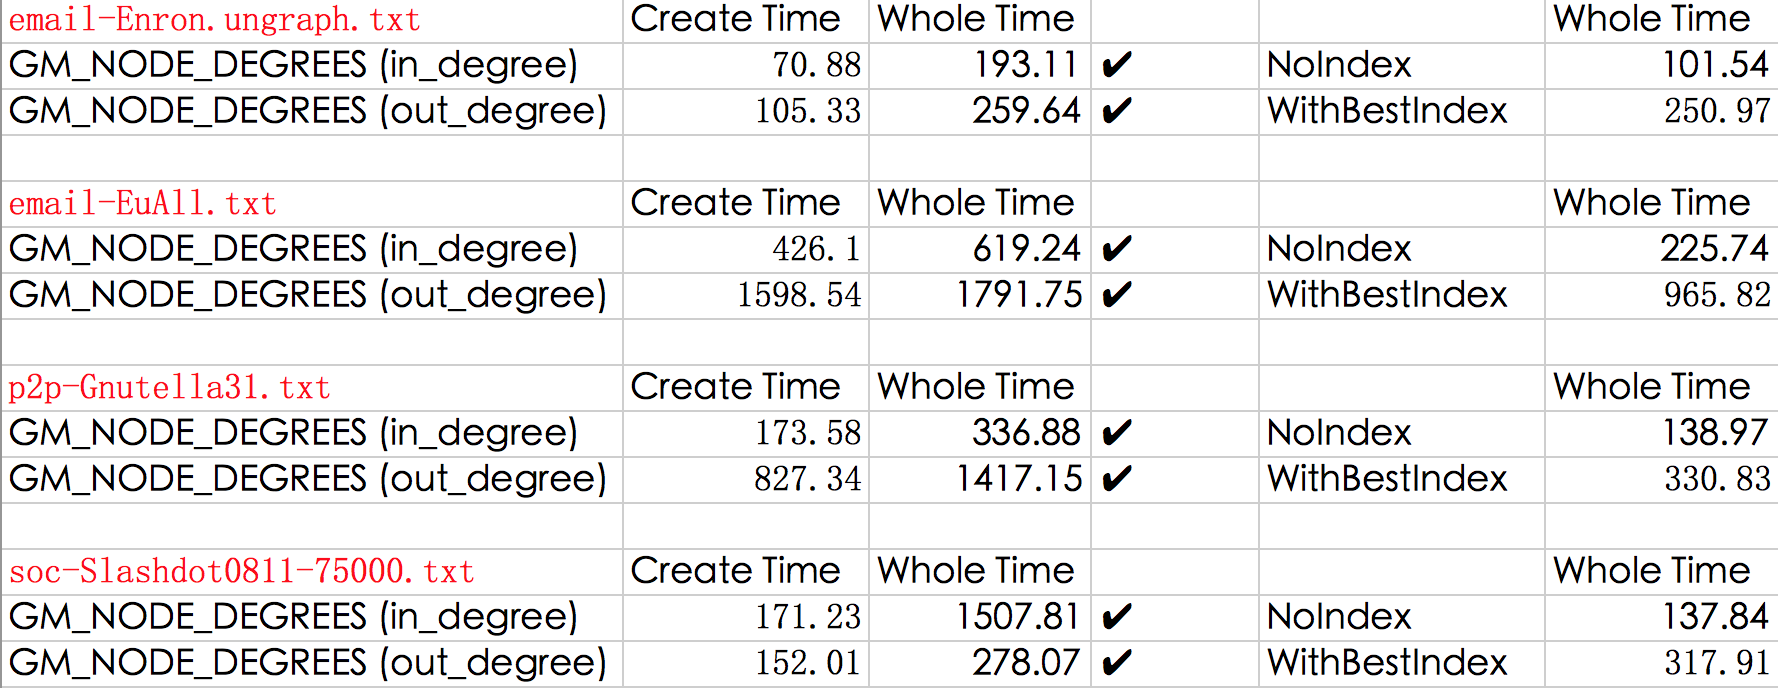
\includegraphics[width=1.0\textwidth]{FIG/DD2.png} \\
\end{tabular}
\caption{Creating Index Experiments on Degree Distribution Algorithm}
\end{center}
\end{figure}

\begin{figure}[H]
\begin{center}
\begin{tabular}{cc}
     % uncomment the next lines, and give the right ps files
     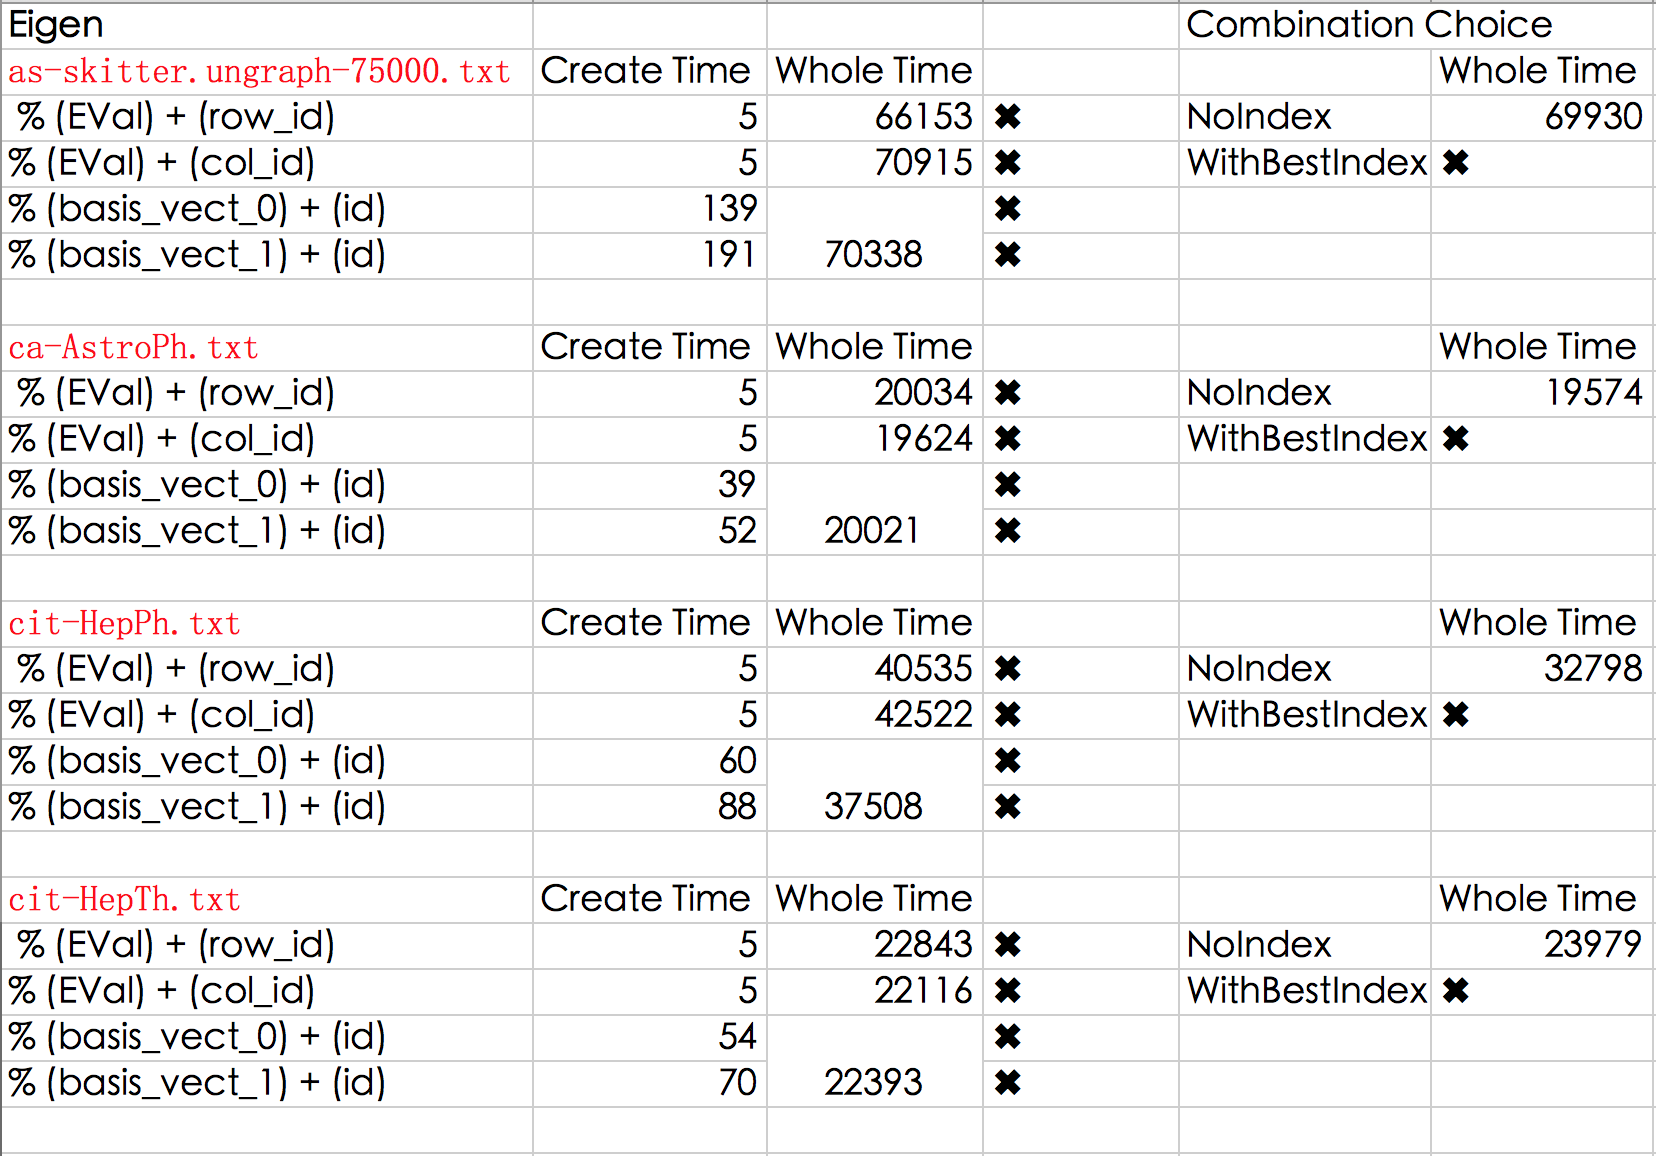
\includegraphics[width=1.0\textwidth]{FIG/Eigen1.png} \\
     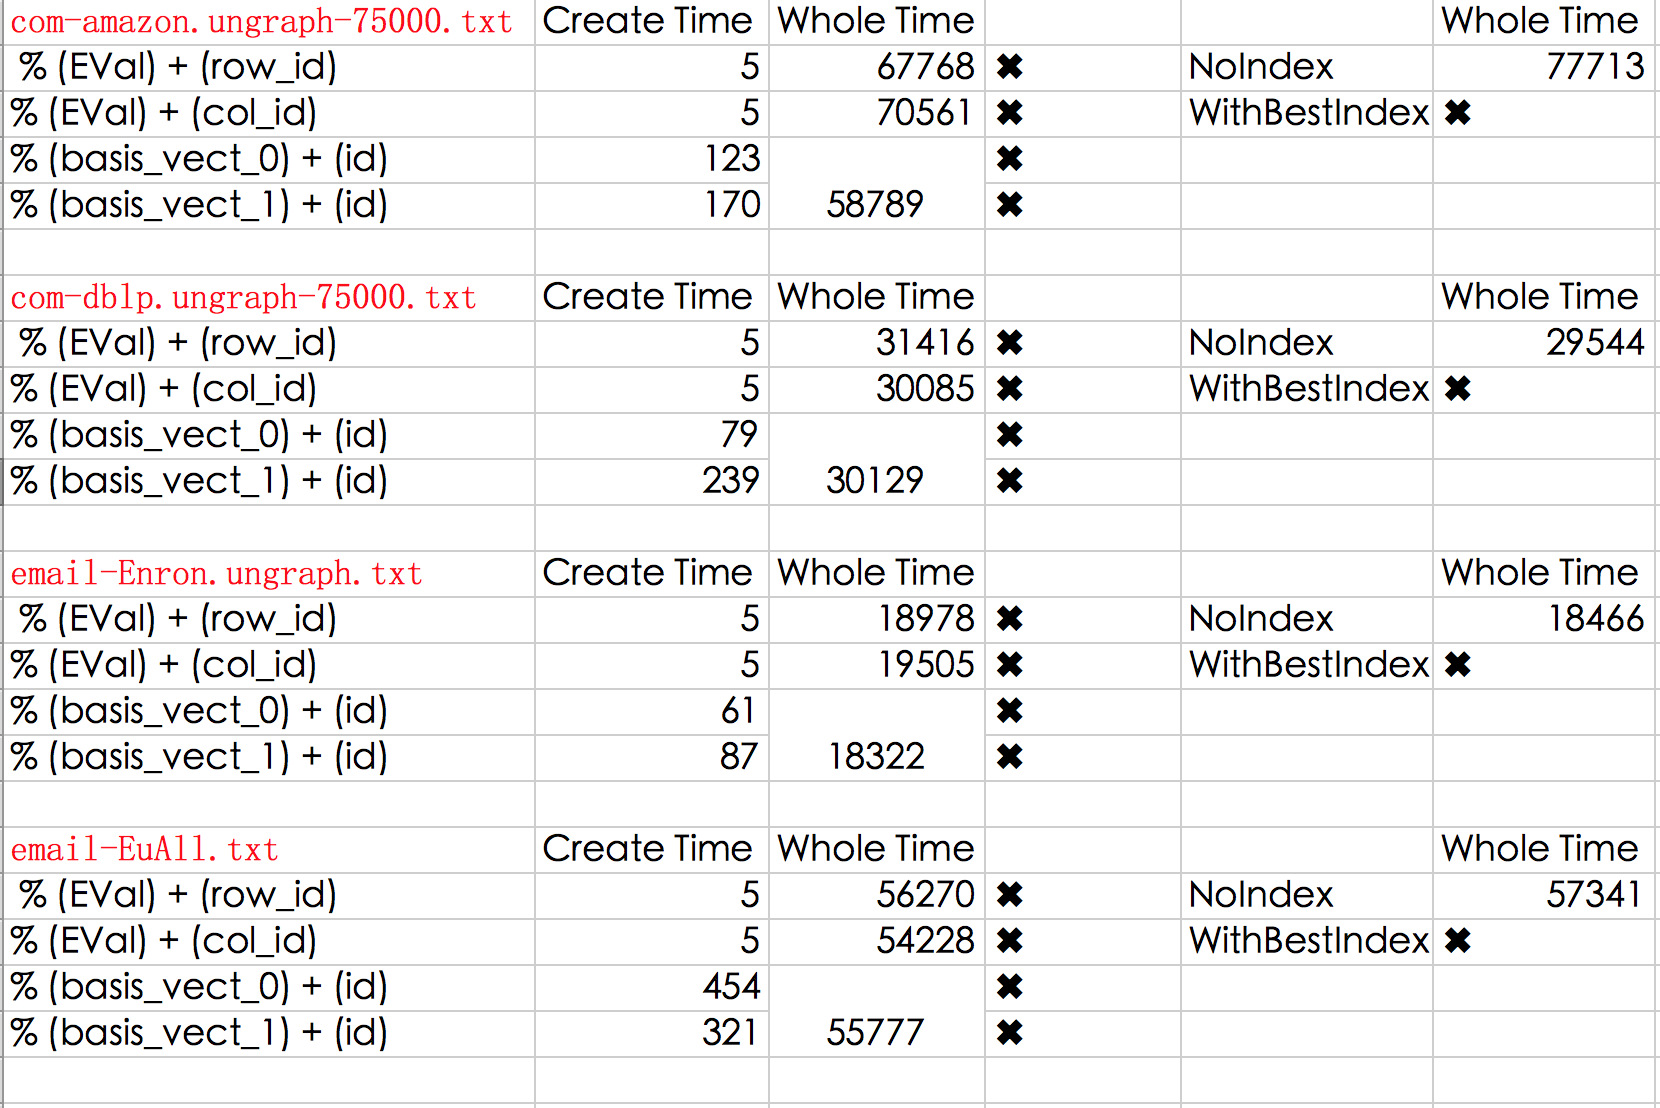
\includegraphics[width=1.0\textwidth]{FIG/Eigen2.png} \\
     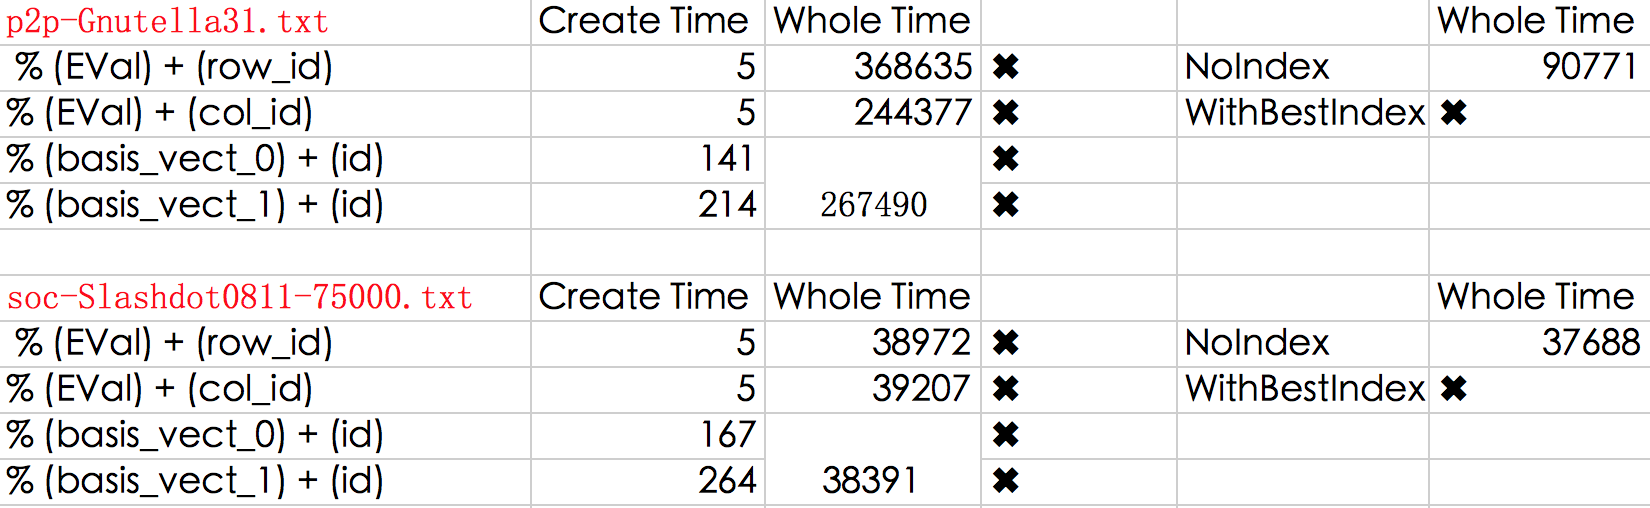
\includegraphics[width=1.0\textwidth]{FIG/Eigen3.png} \\
\end{tabular}
\caption{Creating Index Experiments on Eigen Value Computation Algorithm}
\end{center}
\end{figure}

\begin{figure}[H]
\begin{center}
\begin{tabular}{cc}
     % uncomment the next lines, and give the right ps files
     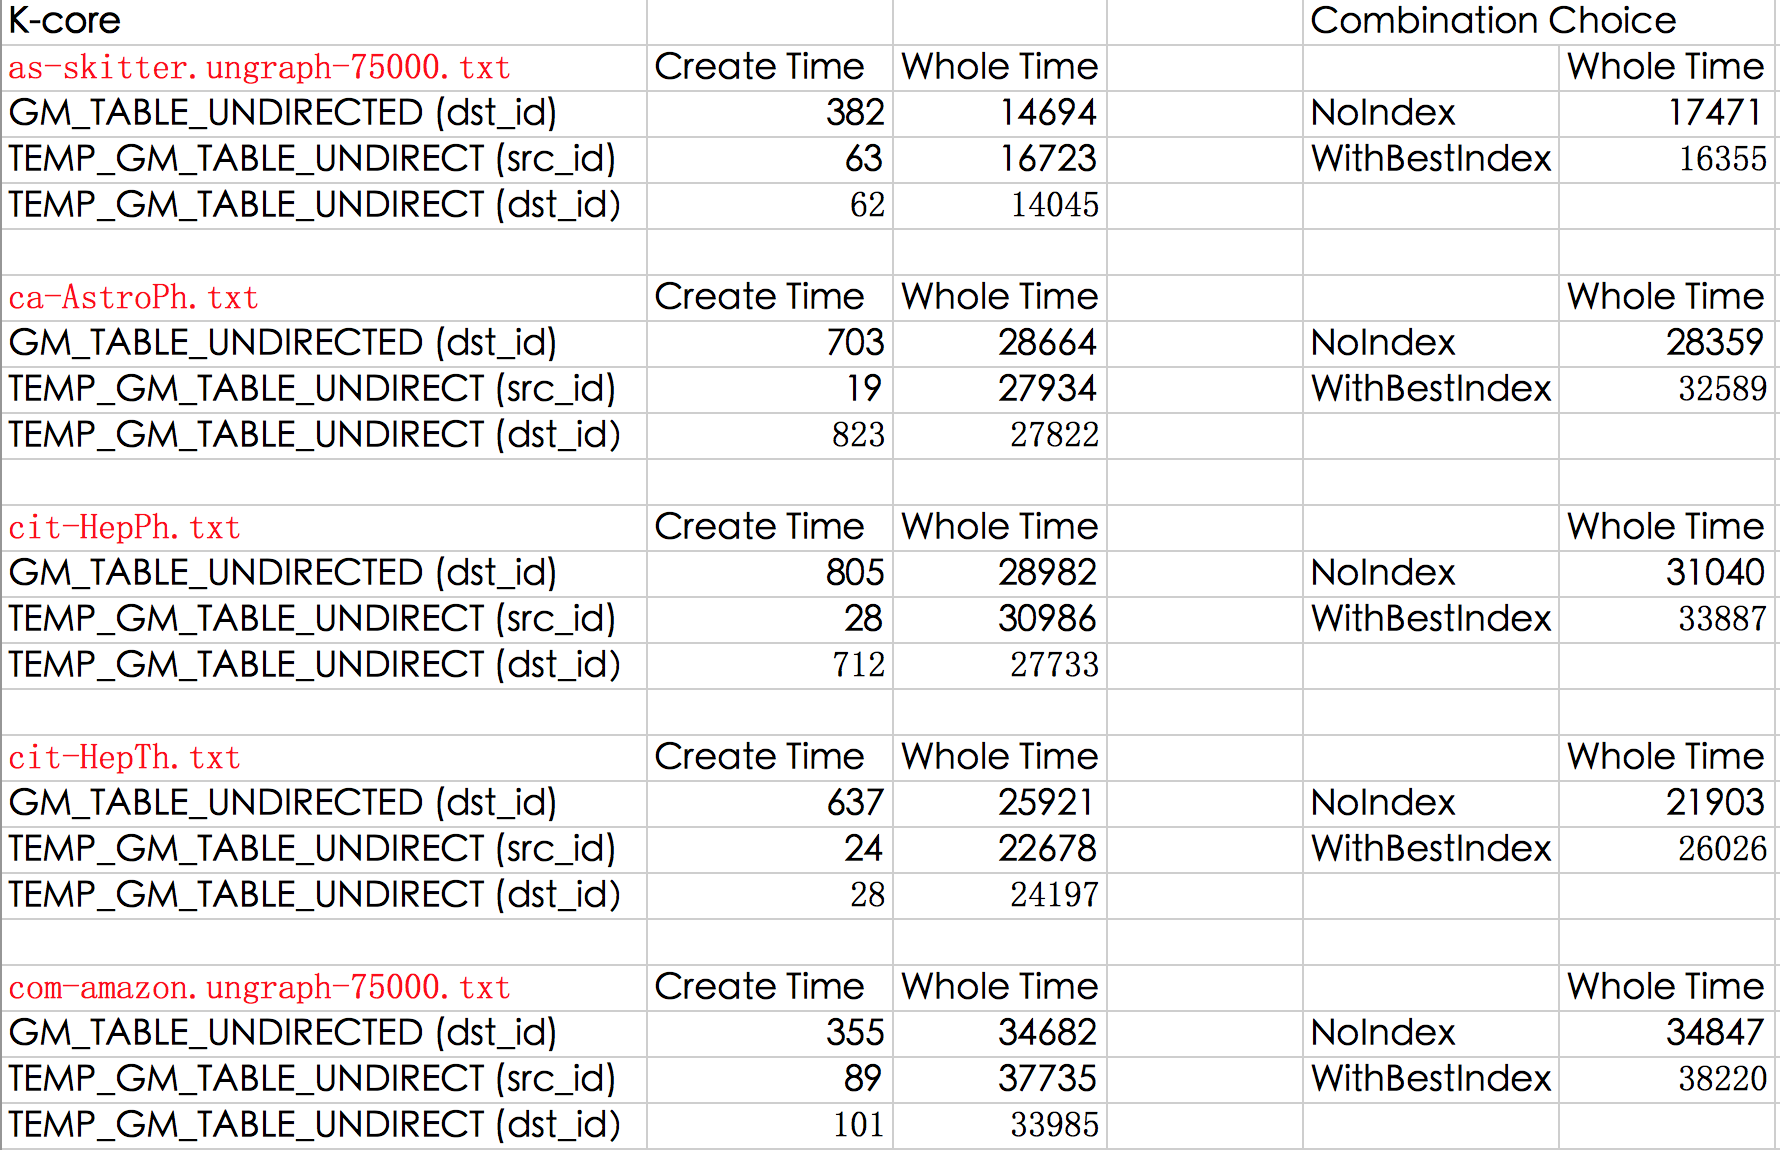
\includegraphics[width=1.0\textwidth]{FIG/KC1.png} \\
     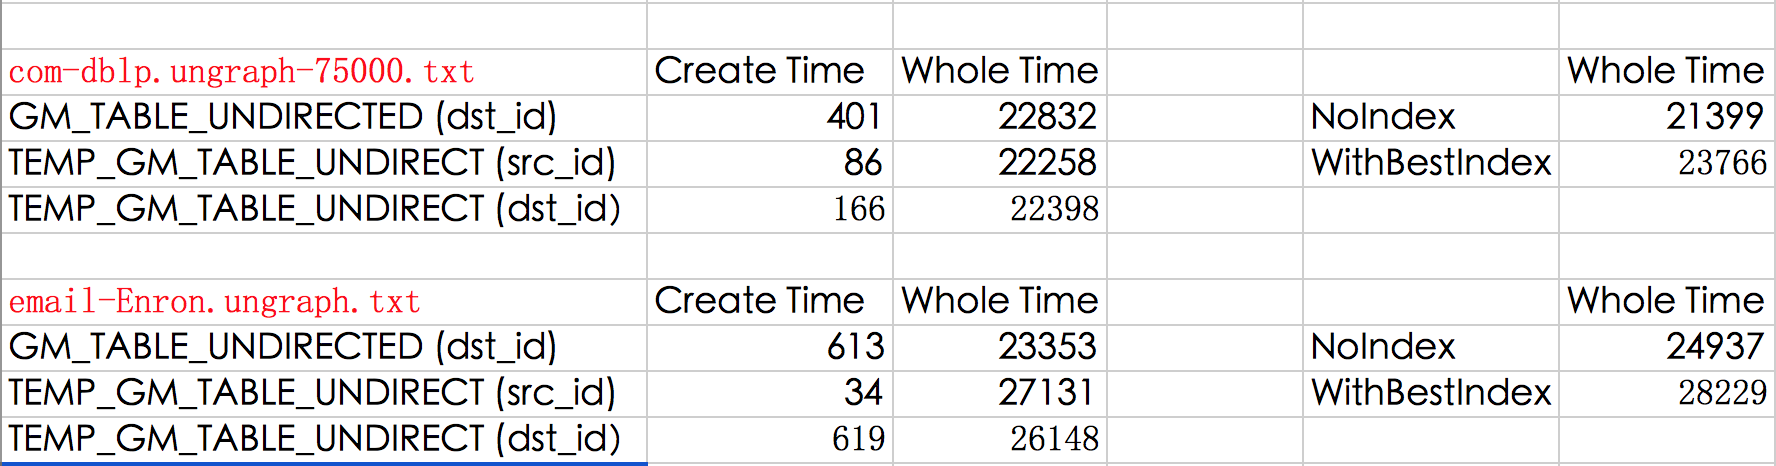
\includegraphics[width=1.0\textwidth]{FIG/KC2.png} \\
\end{tabular}
\caption{Creating Index Experiments on K-core Algorithm}
\end{center}
\end{figure}

\begin{figure}[H]
\begin{center}
\begin{tabular}{cc}
     % uncomment the next lines, and give the right ps files
     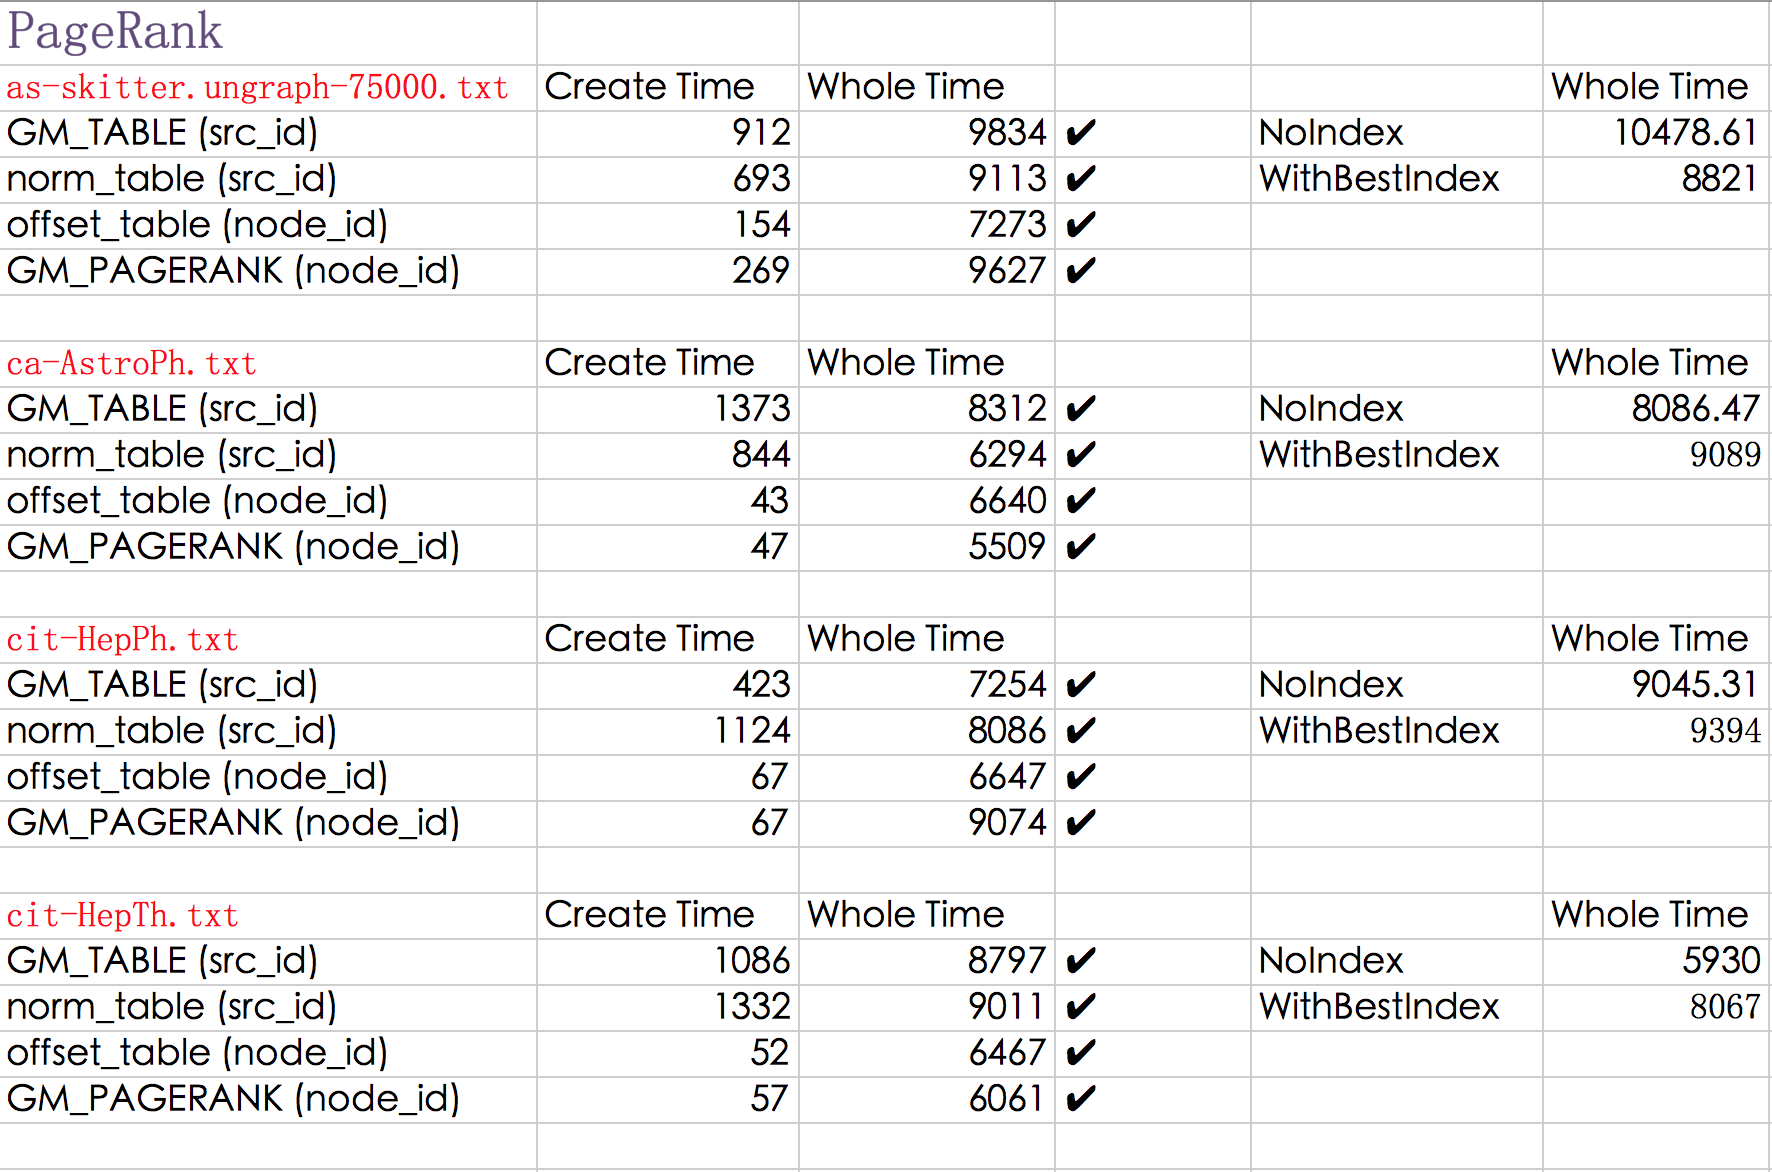
\includegraphics[width=1.0\textwidth]{FIG/PR1.png} \\
     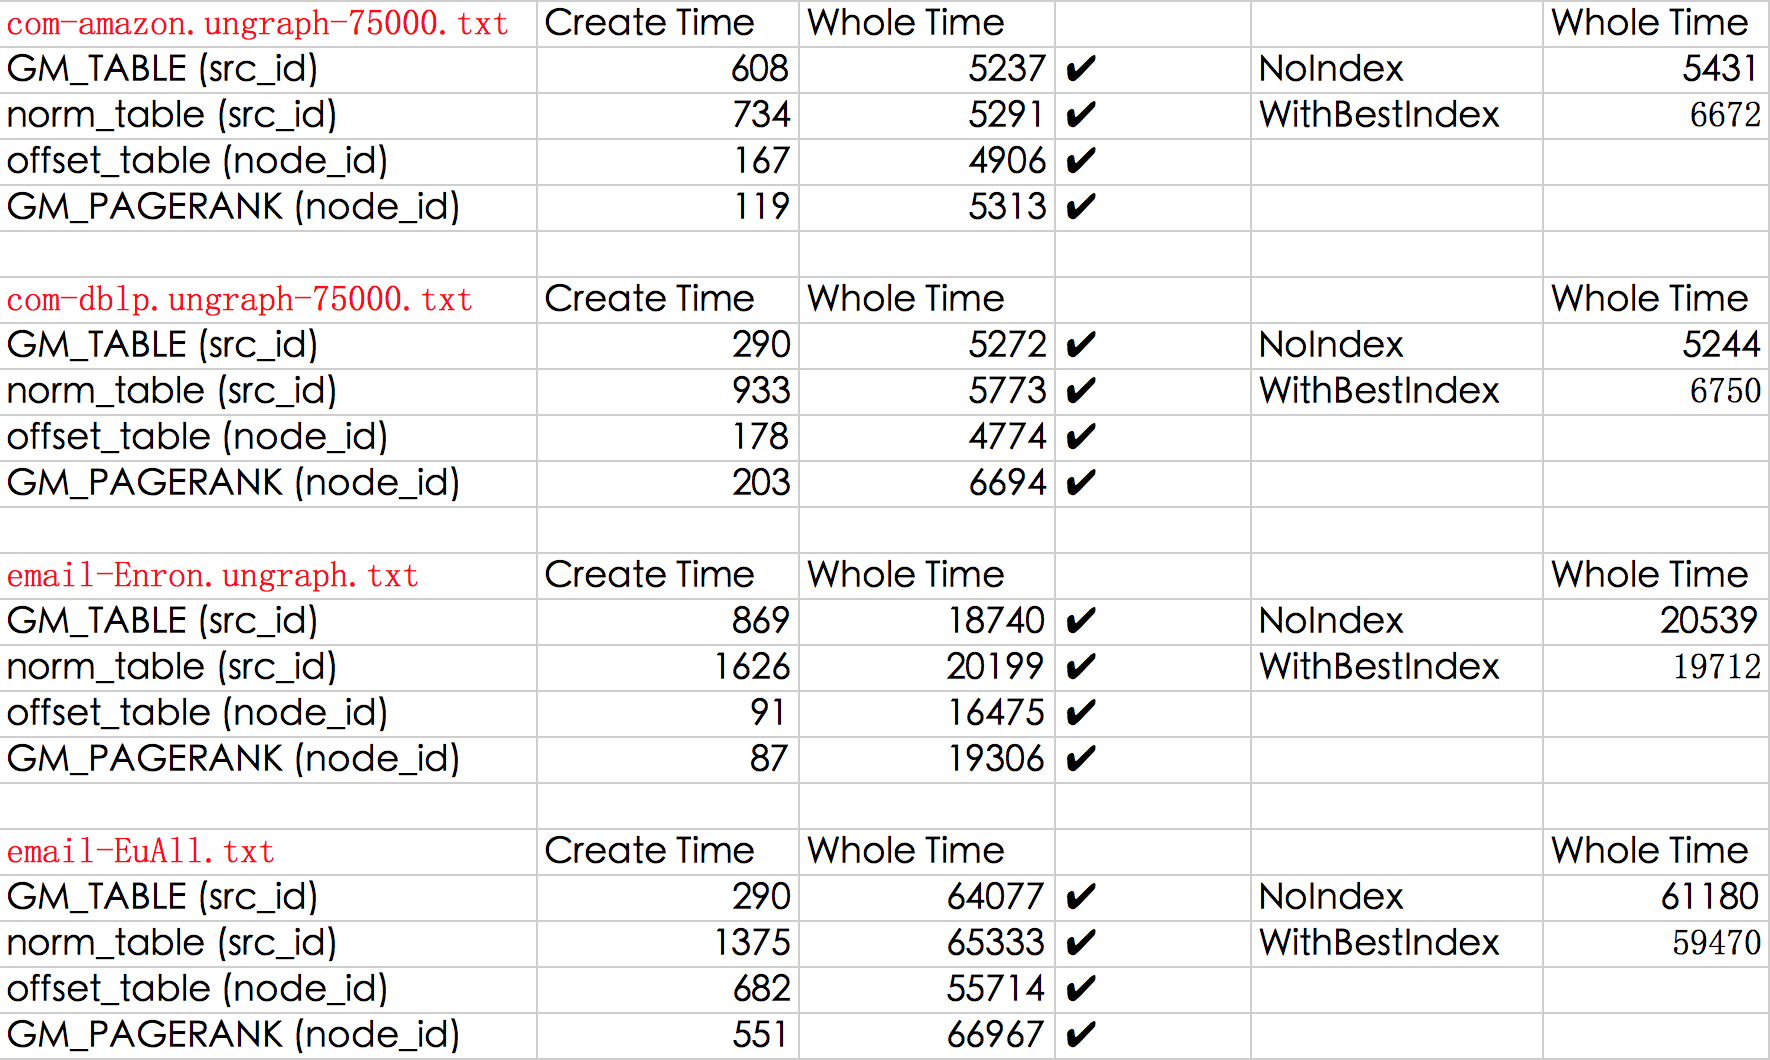
\includegraphics[width=1.0\textwidth]{FIG/PR2.png} \\
\end{tabular}
\caption{Creating Index Experiments on PageRank Algorithm}
\end{center}
\end{figure}


The following are the results of the degree distribution and pagerank results for the ten datasets.
\begin{figure}[H]
\begin{center}
\begin{tabular}{cc}
     % uncomment the next lines, and give the right ps files
     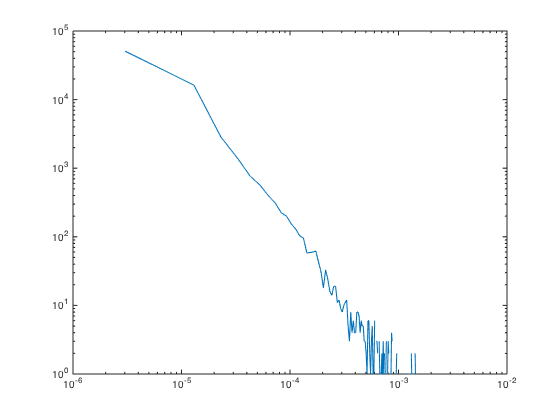
\includegraphics[width=0.3\textwidth]{FIG/1pagerank.png} &
     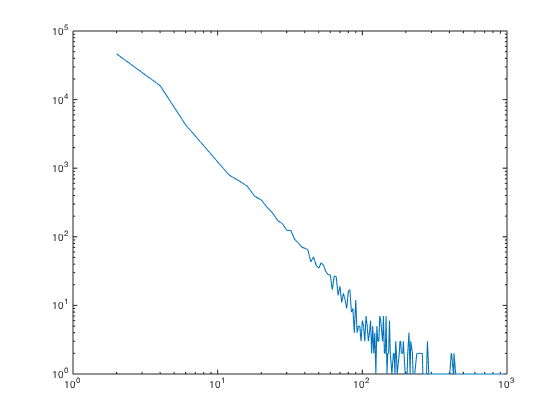
\includegraphics[width=0.3\textwidth]{FIG/1degreedist.png} \\
\end{tabular}
\caption{Result on PageRank Algorithm and Degree Distribution}
\end{center}
\end{figure}

\begin{figure}[H]
\begin{center}
\begin{tabular}{cc}
     % uncomment the next lines, and give the right ps files
     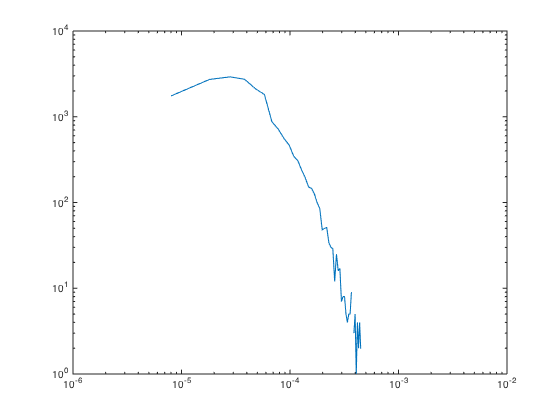
\includegraphics[width=0.3\textwidth]{FIG/2pagerank.png} &
     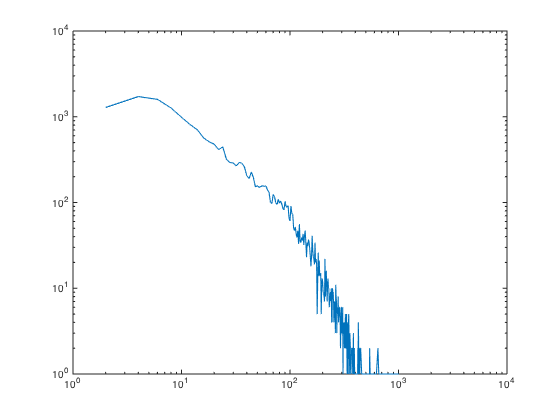
\includegraphics[width=0.3\textwidth]{FIG/2degreedist.png} \\
\end{tabular}
\caption{Result on PageRank Algorithm and Degree Distribution}
\end{center}
\end{figure}

\begin{figure}[H]
\begin{center}
\begin{tabular}{cc}
     % uncomment the next lines, and give the right ps files
     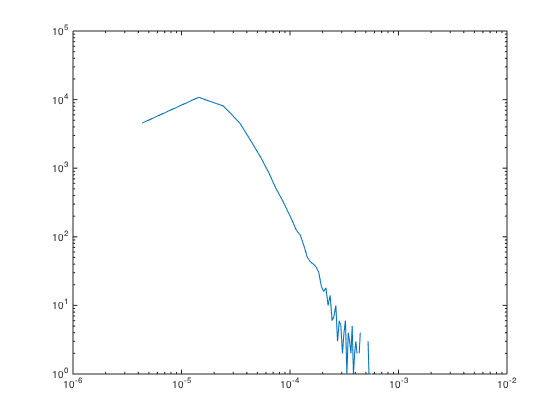
\includegraphics[width=0.3\textwidth]{FIG/3pagerank.png} &
     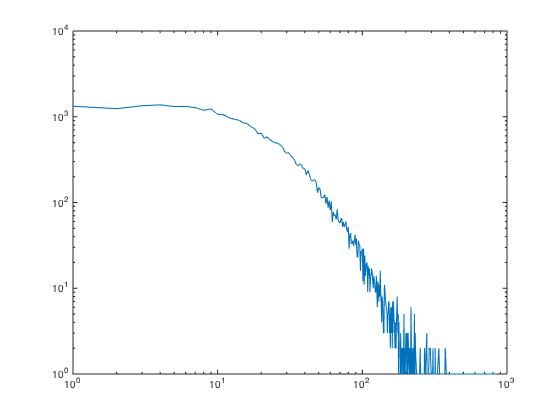
\includegraphics[width=0.3\textwidth]{FIG/3degreedist.png} \\
\end{tabular}
\caption{Result on PageRank Algorithm and Degree Distribution}
\end{center}
\end{figure}

\begin{figure}[H]
\begin{center}
\begin{tabular}{cc}
     % uncomment the next lines, and give the right ps files
     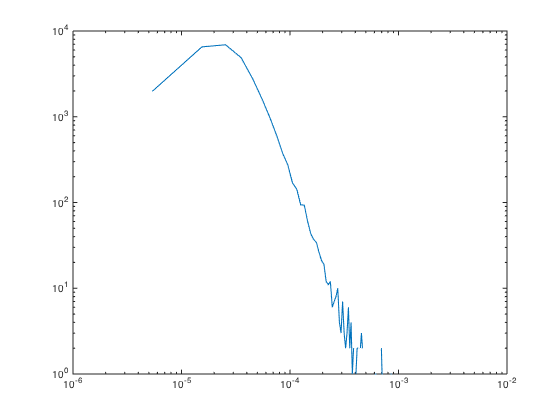
\includegraphics[width=0.3\textwidth]{FIG/4pagerank.png} &
     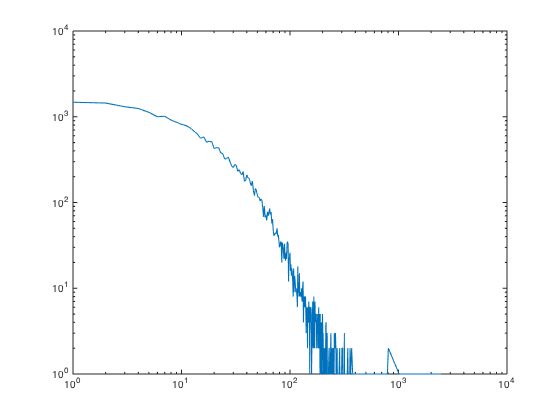
\includegraphics[width=0.3\textwidth]{FIG/4degreedist.png} \\
\end{tabular}
\caption{Result on PageRank Algorithm and Degree Distribution}
\end{center}
\end{figure}

\begin{figure}[H]
\begin{center}
\begin{tabular}{cc}
     % uncomment the next lines, and give the right ps files
     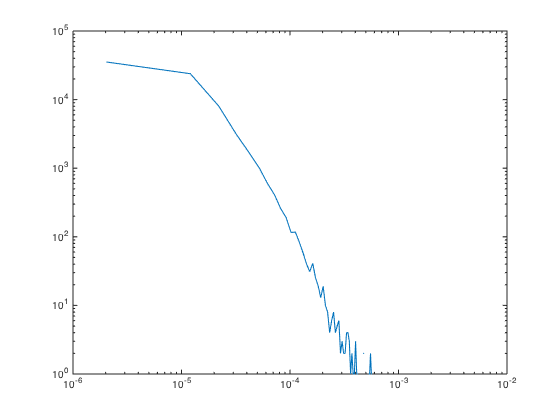
\includegraphics[width=0.3\textwidth]{FIG/5pagerank.png} &
     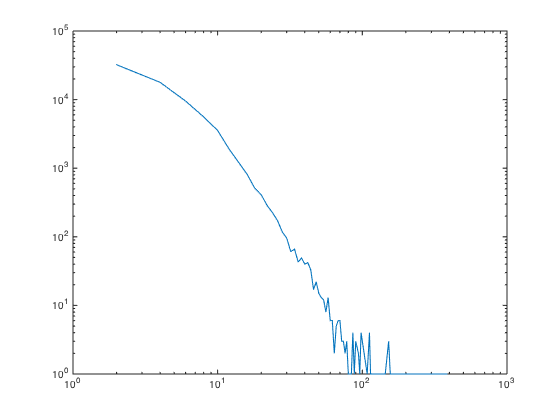
\includegraphics[width=0.3\textwidth]{FIG/5degreedist.png} \\
\end{tabular}
\caption{Result on PageRank Algorithm and Degree Distribution}
\end{center}
\end{figure}

\begin{figure}[H]
\begin{center}
\begin{tabular}{cc}
     % uncomment the next lines, and give the right ps files
     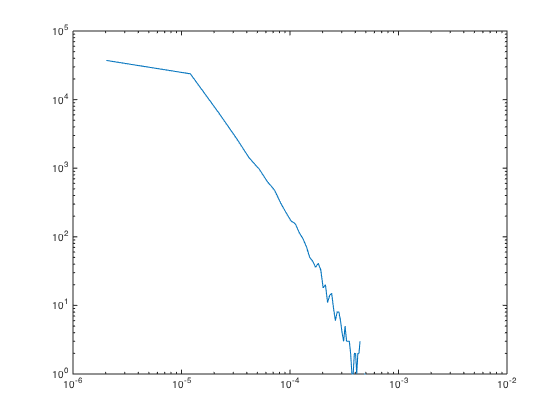
\includegraphics[width=0.3\textwidth]{FIG/6pagerank.png} &
     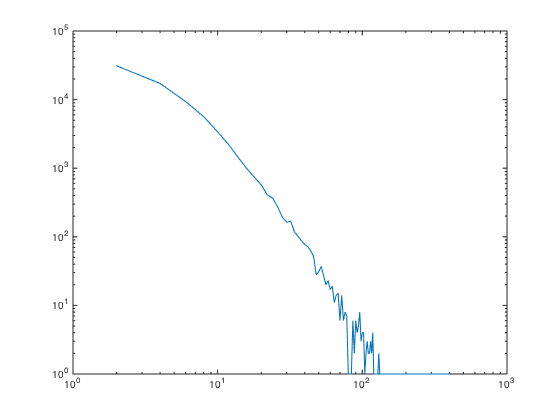
\includegraphics[width=0.3\textwidth]{FIG/6degreedist.png} \\
\end{tabular}
\caption{Result on PageRank Algorithm and Degree Distribution}
\end{center}
\end{figure}

\begin{figure}[H]
\begin{center}
\begin{tabular}{cc}
     % uncomment the next lines, and give the right ps files
     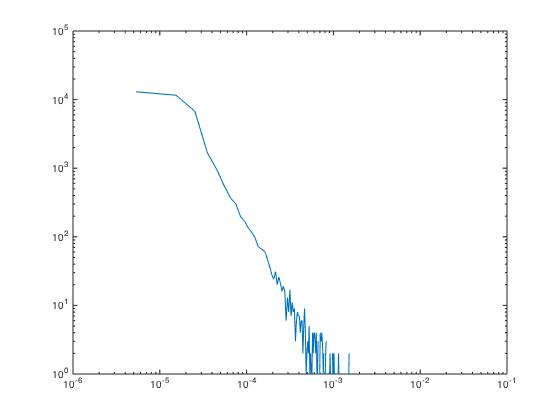
\includegraphics[width=0.3\textwidth]{FIG/7pagerank.png} &
     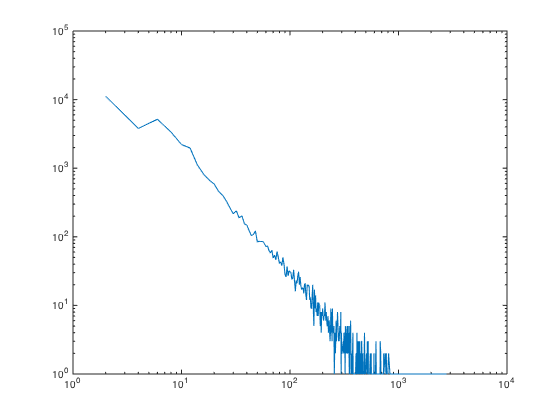
\includegraphics[width=0.3\textwidth]{FIG/7degreedist.png} \\
\end{tabular}
\caption{Result on PageRank Algorithm and Degree Distribution}
\end{center}
\end{figure}

\begin{figure}[H]
\begin{center}
\begin{tabular}{cc}
     % uncomment the next lines, and give the right ps files
     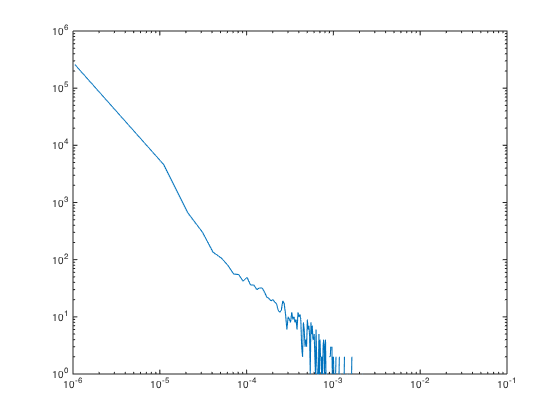
\includegraphics[width=0.3\textwidth]{FIG/8pagerank.png} &
     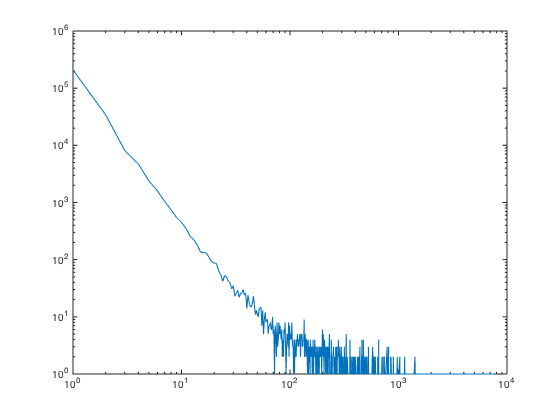
\includegraphics[width=0.3\textwidth]{FIG/8degreedist.png} \\
\end{tabular}
\caption{Result on PageRank Algorithm and Degree Distribution}
\end{center}
\end{figure}

\begin{figure}[H]
\begin{center}
\begin{tabular}{cc}
     % uncomment the next lines, and give the right ps files
     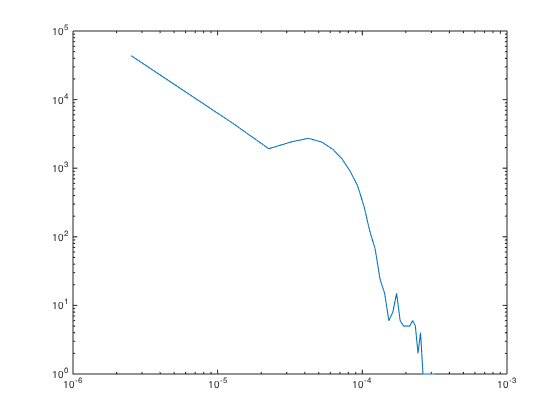
\includegraphics[width=0.3\textwidth]{FIG/9pagerank.png} &
     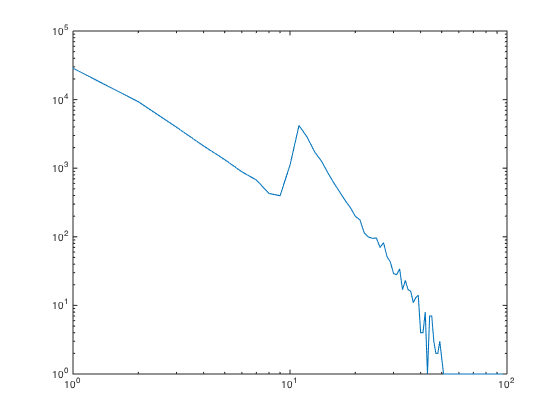
\includegraphics[width=0.3\textwidth]{FIG/9degreedist.png} \\
\end{tabular}
\caption{Result on PageRank Algorithm and Degree Distribution}
\end{center}
\end{figure}

\begin{figure}[H]
\begin{center}
\begin{tabular}{cc}
     % uncomment the next lines, and give the right ps files
     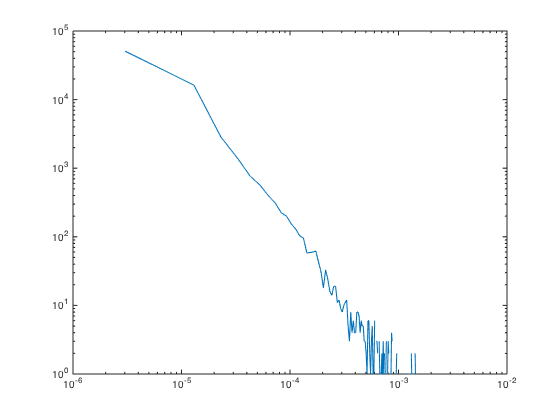
\includegraphics[width=0.3\textwidth]{FIG/1pagerank.png} &
     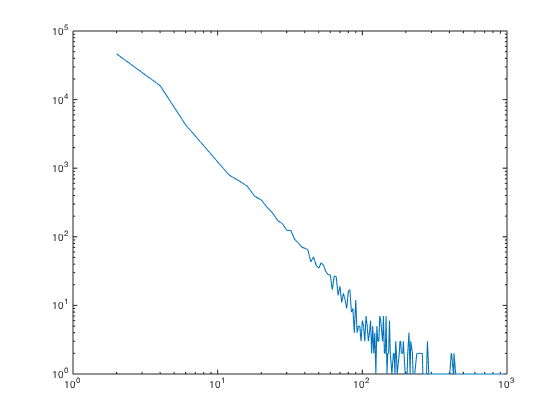
\includegraphics[width=0.3\textwidth]{FIG/1degreedist.png} \\
\end{tabular}
\caption{Result on PageRank Algorithm and Degree Distribution}
\end{center}
\end{figure}

\begin{figure}[H]
\begin{center}
\begin{tabular}{cc}
     % uncomment the next lines, and give the right ps files
     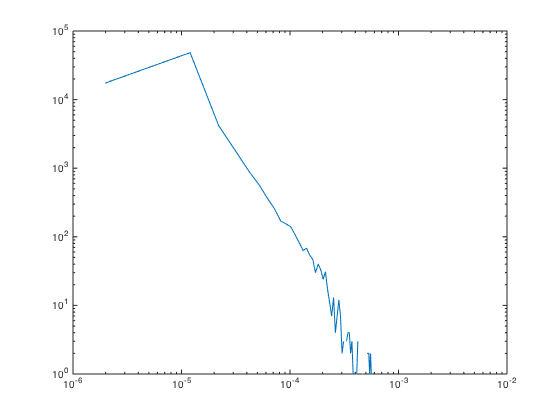
\includegraphics[width=0.3\textwidth]{FIG/10pagerank.png} &
     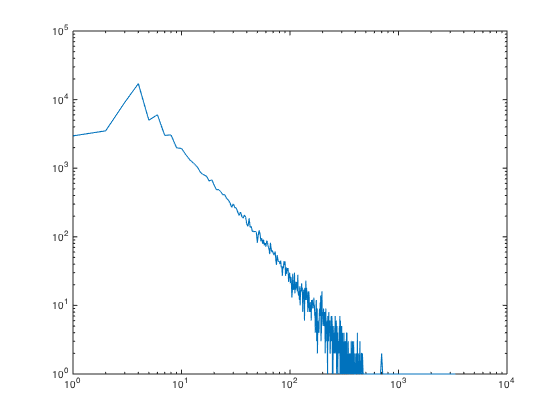
\includegraphics[width=0.3\textwidth]{FIG/10degreedist.png} \\
\end{tabular}
\caption{Result on PageRank Algorithm and Degree Distribution}
\end{center}
\end{figure}